\documentclass{beamer}

\usepackage{amsmath}
\usepackage{amssymb}
\usepackage{mathtools}
%\usepackage{float}
\usepackage[pdftex]{graphicx}
%\usepackage{ngerman}
\usepackage[T1]{fontenc}
\usepackage[utf8]{inputenc}
\usepackage{enumerate}
\usepackage{ifpdf}

\usetheme{Warsaw}

\title{Elektronikpraktikum Auswertung: Versuch 2}
\author{Gruppe 1 \\ Patrick Heuer \\ Benjamin Lotter}
\date{}

\begin{document}
\maketitle
%\tableofcontents

\section{Digital-zu-Analog-Wandler (DAC)} % (fold)
\label{sec:Digital-zu-Analog-Wandler_(DAC)}

\subsection{R-2R-Netzwerk} % (fold)
\label{sub:R-2R-Netzwerk}
\begin{frame}
    \frametitle{R-2R-Netzwerk}
    \framesubtitle{}
    \begin{figure}[H]
        \begin{center}
        %        \includegraphics[scale=0.2]{./img/schaltung/r2r_0.png}
        \end{center}
    \end{figure}
\end{frame}

\begin{frame}
    \frametitle{Funktionsweise}
    \framesubtitle{}
    \begin{columns}[c]
        \column{0.7\textwidth}
            lol    
        \column{0.3\textwidth}
            \begin{figure}[H]
                 \begin{center}
                 %        \includegraphics[scale=0.2]{./img/schaltung/r2r_0.png}
                 \end{center}
            \end{figure}
    \end{columns}
\end{frame}
% subsection R-2R-Netzwerk (end)

\subsection{DAC-Chip DAC0909} % (fold)
\label{sub:DAC-Chip_DAC0909}

% subsection DAC-Chip DAC0909 (end)

% section Digital-zu-Analog-Wandler (DAC) (end)

\section{Invertierender Verstärker} % (fold)
\label{sec:Invertierender_Verstärker}
% section Invertierender Verstärker (end)

\section{Sequentielle Logik} % (fold)
\label{sec:Sequentielle Logik}
\subsection{RS-Flipflop} % (fold)
\label{sub:RS-Flipflop}
\begin{frame}
    \frametitle{RS-Flipflop}
    \framesubtitle{}
    \begin{figure}[H]
    \begin{center}
            \includegraphics[scale=0.5]{./img/schaltung/RS-FF.png}
    \end{center}
    \end{figure}
\end{frame}
\begin{frame}
    \frametitle{Funktionsweise}
    \framesubtitle{}
    \begin{columns}[c]
        \column{0.6\textwidth}
            \boxed{
                \begin{tabular}{c|c||c}
                    $\bar{S}$ & $\bar{R}$ & Q \\
                    \hline
                    1 & 1 & unverändert \\
                    0 & 1 & 1 (gesetzt) \\
                    1 & 0 & 0 (zurückgesetzt) \\
                    0 & 0 & Glitch ($Q = \bar{Q}$)
                \end{tabular}
                }
            \begin{block}{Gleizeitiges Auslößen}
                \begin{itemize}
                    \item ????
                \end{itemize}
            \end{block}
        \column{0.4\textwidth}
            \begin{figure}[H]
            \begin{center}
                    \includegraphics[scale=0.5]{./img/schaltung/RS-FF.png}
            \end{center}
            \end{figure}
    \end{columns}
\end{frame}
% subsection RS-Flipflop (end)

\subsection{Taktgesteuertes RS-Flip-Flop} % (fold)
\label{sub:Taktgesteuertes RS-Flip-Flop}
\begin{frame}
    \frametitle{Taktgesteuertes RS-Flip-Flop}
    \framesubtitle{}
     \begin{figure}[H]
     \begin{center}
             \includegraphics[scale=0.6]{./img/schaltung/RS-FF-T.png}
     \end{center}
     \end{figure}
\end{frame}
\begin{frame}
    \frametitle{Funktionsweise}
    \framesubtitle{}
    \begin{columns}[c]
        \column{0.6\textwidth}
            \boxed{
                \begin{tabular}{c|c|c||c}
                    S & R & C & Q \\
                    \hline
                     0 & 0 & 0 & unverändert \\
                     0 & 1 & 0 & unverändert \\
                     1 & 0 & 0 & unverändert \\
                     1 & 1 & 0 & unverändert \\
                     \hline
                     0 & 0 & 1 & unverändert \\
                     0 & 1 & 1 & 0 (zurückgesetzt) \\
                     1 & 0 & 1 & 1 (gesetzt) \\
                     1 & 1 & 1 & Glitch ($\bar{Q} = Q$)
                \end{tabular}
            }
        \column{0.4\textwidth}
             \begin{figure}[H]
             \begin{center}
                     \includegraphics[scale=0.6]{./img/schaltung/RS-FF-T.png}
             \end{center}
             \end{figure}
             \begin{figure}[H]
             \begin{center}
                     \includegraphics[scale=0.32]{./img/Aufgabe_2_b.eps}
             \end{center}
             \end{figure}
    \end{columns}
\end{frame}
% subsection Taktgesteuertes RS-Flip-Flop (end)

\subsection{D-Latch} % (fold)
\label{sub:D-Latch}
\begin{frame}
    \frametitle{D-Latch}
    \framesubtitle{}
    \begin{figure}[H]
    \begin{center}
            \includegraphics[scale=0.6]{./img/schaltung/D-Latch.png}
    \end{center}
    \end{figure}
\end{frame}
\begin{frame}
    \frametitle{Funktionsweise}
    \framesubtitle{}
    \begin{columns}[c]
        \column{0.6\textwidth}
            bla 
        \column{0.4\textwidth}
            \begin{figure}[H]
            \begin{center}
                    \includegraphics[scale=0.6]{./img/schaltung/D-Latch.png}
            \end{center}
            \end{figure}
            \begin{figure}[H]
            \begin{center}
                    \includegraphics[scale=0.3]{./img/Aufgabe_2_c.eps}
            \end{center}
            \end{figure}
    \end{columns}
\end{frame}
% subsection D-Latch (end)

\subsection{Flankengetriggertes D-Latch} % (fold)
\label{sub:Flankengetriggertes D-Latch}
\begin{frame}
    \frametitle{Flankengetriggertes D-Latch}
    \framesubtitle{}
     \begin{figure}[H]
     \begin{center}
             \includegraphics[scale=0.3]{./img/schaltung/flanken_d.png}
     \end{center}
     \end{figure}
\end{frame}
\begin{frame}
    \frametitle{Flankengetriggertes D-Latch}
    \framesubtitle{}
     \begin{columns}[c]
         \column{0.6\textwidth}
         \begin{figure}[H]
         \begin{center}
                 \includegraphics[scale=0.25]{./img/schaltung/flanken_d.png}
         \end{center}
         \end{figure}
         \column{0.4\textwidth}
         \begin{figure}[H]
         \begin{center}
                 \includegraphics[scale=0.3]{./img/Aufgabe_3_d.eps}
         \end{center}
         \end{figure}
     \end{columns}
     \begin{block}{Funktionsweise}
        \begin{itemize}
            \item Clock muss vor Triggerung auf 1 stehen 
            \item Flanken werden nicht erkannt
        \end{itemize}
     \end{block}
\end{frame}
% subsection Flankengetriggertes D-Latch (end)

% section Sequentielle Logik (end)

\section{Zähler} % (fold)
\label{sec:Zähler}
\begin{frame}
    \frametitle{Zähler}
    \framesubtitle{}
     \begin{figure}[H]
     \begin{center}
             \includegraphics[scale=0.3]{./img/schaltung/zahler.png}
     \end{center}
     \end{figure}
\end{frame}
\begin{frame}
    \frametitle{Entwicklung}
    \framesubtitle{}
    \begin{columns}[c]
        \column{0.5\textwidth}
         \begin{block}{Funktionsweise}
            \begin{itemize}
                \item D-Latch flipt aktuelles Bit 
                \item falls Q gesetzt wird $\bar{Q}$ und somit der nächste D-Latch
                gesetzt
                \item Zahl muss 'rückwärts' gelesen werden
            \end{itemize}
         \end{block}
        \column{0.5\textwidth}
             \begin{center}
                \boxed{
                    \begin{tabular}{c}
                        0000 \\
                        1000 \\
                        0100 \\
                        1100 \\
                        0010 \\
                        1010 \\
                        1110 \\
                        0001 \\
                        1001 \\
                        0101 \\
                        1101 \\
                        0011 \\
                        1011 \\
                        0111 \\
                        1111 \\
                    \end{tabular}
                }
             \end{center}
    \end{columns}
\end{frame}
% section Zähler (end)

\begin{frame}
    \frametitle{Aufgabe 5}
    \framesubtitle{}
    \begin{itemize}
        \item Untersuchung des Signalverhaltens bei Koaxialkabeln
    \end{itemize}
\end{frame}
\begin{frame}
    \frametitle{Aufgabe 5}
    \framesubtitle{Signalgeschwindigkeit}
    \begin{itemize}
        \item Kabelende wird offen gelassen
        \item Beobachtung: Zwei Pulse hintereinander durch Signalreflexion am
        offenen Kabelende
    \end{itemize}
    \begin{figure}[H]
    \begin{center}
            \includegraphics[scale=0.2]{./img/5a.png}
    \end{center}
    \end{figure}
\end{frame}
\begin{frame}
    \frametitle{Aufgabe 5}
    \framesubtitle{Signalgeschwindigkeit}
    \begin{itemize}
        \item Signal wird am offenen Kabelende reflektiert
        \item Signalgeschwindigkeit: $ v = \frac{20m}{100ns}=2 \cdot 10^8
        ms^{-1}$
    \end{itemize}
\end{frame}
\begin{frame}
    \frametitle{Aufgabe 5}
    \framesubtitle{Abschlusswiderstand}
    \begin{itemize}
        \item Kabelende wird mit Potentiometer abgeschlossen
        \item Widerstand wird variiert
    \end{itemize}
    \begin{figure}[H]
    \begin{center}
            \includegraphics[scale=0.2]{./img/5b_Potentiometer_1.png}
    \end{center}
    \end{figure}
\end{frame}
\begin{frame}
    \frametitle{Aufgabe 5}
    \framesubtitle{Abschlusswiderstand}
    \begin{itemize}
        \item Kabelende wird mit Potentiometer abgeschlossen
        \item Widerstand wird variiert
    \end{itemize}
    \begin{figure}[H]
    \begin{center}
            \includegraphics[scale=0.2]{./img/5b_Potentiometer_3.png}
    \end{center}
    \end{figure}
\end{frame}
\begin{frame}
    \frametitle{Aufgabe 5}
    \framesubtitle{Abschlusswiderstand}
    \begin{itemize}
        \item Kabelende wird mit Potentiometer abgeschlossen
        \item Widerstand wird variiert
    \end{itemize}
    \begin{figure}[H]
    \begin{center}
            \includegraphics[scale=0.2]{./img/5b_Potentiometer_2.png}
    \end{center}
    \end{figure}
    \begin{itemize}
        \item Auslöschung des Signals bei $R=53.62 \Omega$
    \end{itemize}
\end{frame}
\begin{frame}
    \frametitle{Aufgabe 5}
    \framesubtitle{Abschlusswiderstand}
    \begin{itemize}
        \item Kabel wird mit $50 \Omega$ abgeschlossen $\rightarrow$
        Auslöschung des Signals
    \end{itemize}
    \begin{figure}[H]
    \begin{center}
            \includegraphics[scale=0.2]{./img/5b_Abschluss.png}
    \end{center}
    \end{figure}
\end{frame}
\begin{frame}
    \frametitle{Aufgabe 5}
    \framesubtitle{Abschlusswiderstand}
    \begin{itemize}
        \item Abschlusswiderstand kann Signal abdämpfen und auslöschen
        \item längere Impulssignale können sich überlagern 
    \end{itemize}
    \begin{center}
    \begin{tabular}{c|c c}
    & Messwerte & Datenblatt \\
    \hline
    v & $2 \cdot 10^{8} ms^{-1}$ & $2 \cdot 10^{8} ms^{-1}$ \\
    C'& $93.249 pFm^{-1}$&$100.7 pFm^{-1}$ \\
    L'& $268.1 nHm^{-1}$& keine Angabe \\
    R & $53.62 \Omega$& $50 \Omega$
    \end{tabular}
    \end{center}
\end{frame}
\begin{frame}
    \frametitle{Aufgabe 5}
    \framesubtitle{Einfache Laufzeit}
    \begin{itemize}
        \item Kabel wird an Kanal des Oszilloskops angeschlossen
    \end{itemize}
    \begin{figure}[H]
    \begin{center}
            \includegraphics[scale=0.2]{./img/5c_zweiter_Kanal.png}
    \end{center}
    \end{figure}
\end{frame}
\begin{frame}
    \frametitle{Aufgabe 5}
    \framesubtitle{Einfache Laufzeit}
    \begin{figure}[H]
    \begin{center}
            \includegraphics[scale=0.2]{./img/5c_zweiter_Kanal.png}
    \end{center}
    \end{figure}
    \begin{itemize}
        \item Erklärung:
        \begin{itemize}
            \item Kabel kommt an Kanal 1 an (gelb)
            \item Kabel kommt an Kanal 2 an (grün)
            \item Kabel wird an Kanal 2 reflektiert und wird in Kanal 1 (gelb)
            gemessen
        \end{itemize}
    \end{itemize}
\end{frame}
\begin{frame}
    \frametitle{Aufgabe 5}
    \framesubtitle{Einfache Laufzeit}
    \begin{itemize}
        \item Kanal 2 wird mit Abschlusswiderstand abgeschlossen
    \end{itemize}
    \begin{figure}[H]
    \begin{center}
            \includegraphics[scale=0.2]{./img/5c_zweiterKanal_Abschlusswiserstand_1.png}
    \end{center}
    \begin{itemize}
        \item Abschlusswiderstand löscht Signal aus $\rightarrow$ keine
        Reflexion
    \end{itemize}
    \end{figure}
\end{frame}
\begin{frame}
    \frametitle{Aufgabe 5}
    \framesubtitle{Dämpfung}
    \begin{itemize}
        \item $100m$ Kabel wird mit Sinusspannung untersucht
    \end{itemize}
\end{frame}
\begin{frame}
    \frametitle{Aufgabe 5}
    \framesubtitle{Dämpfung}
    \begin{figure}[H]
    \begin{center}
            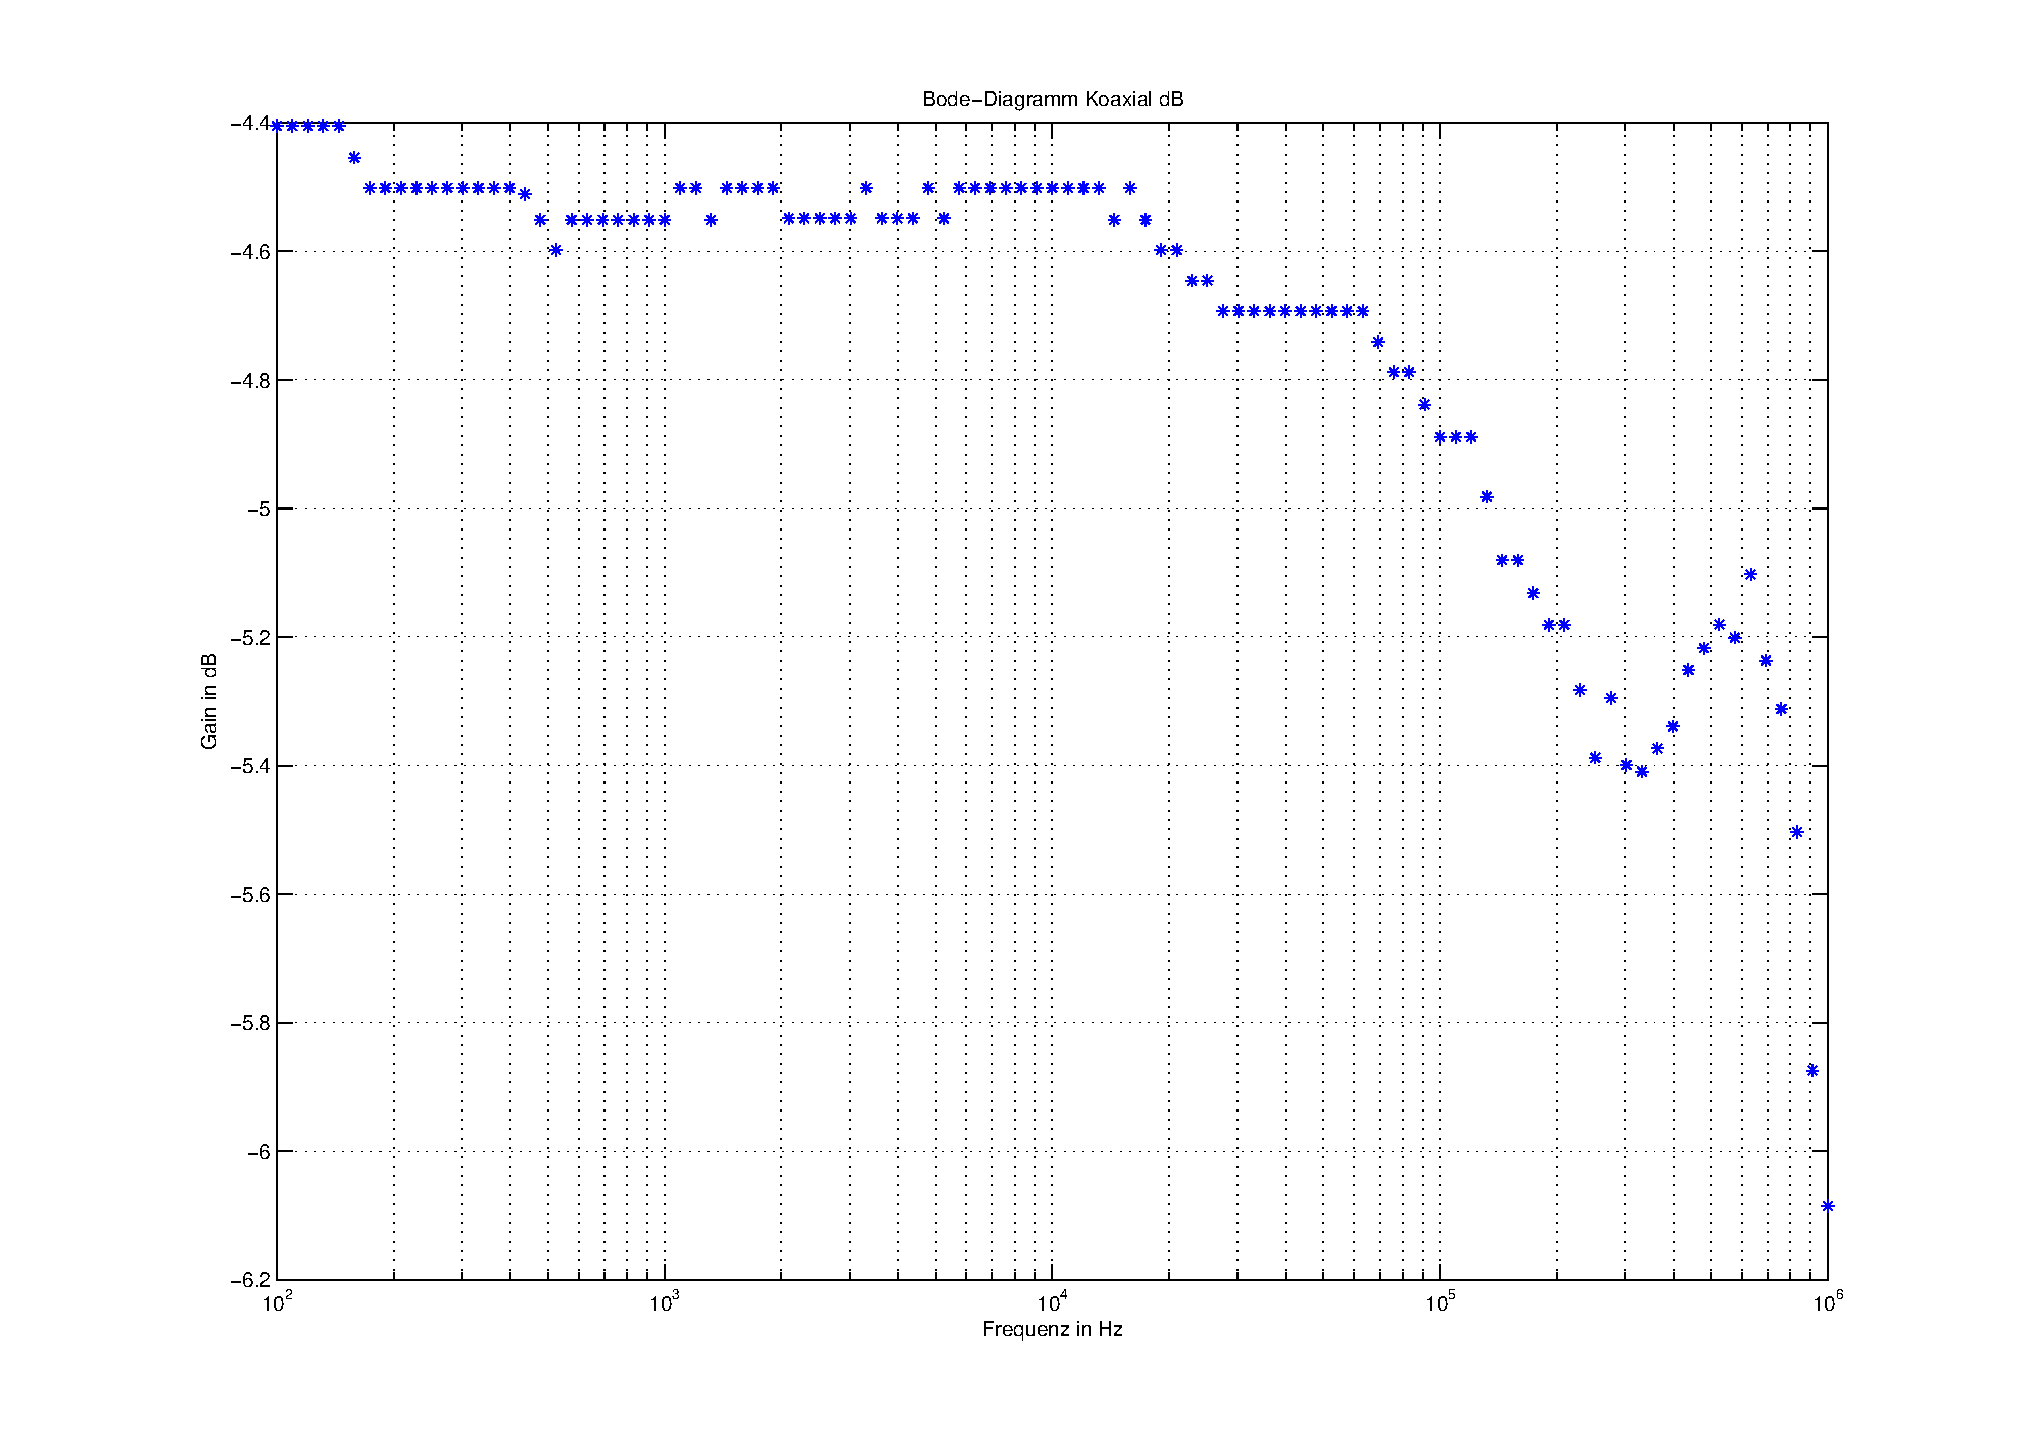
\includegraphics[scale=0.6]{./img/5d_bode_dB.eps}
    \end{center}
    \end{figure}
\end{frame}
\begin{frame}
    \frametitle{Aufgabe 5}
    \framesubtitle{Dämpfung}
    \begin{figure}[H]
    \begin{center}
            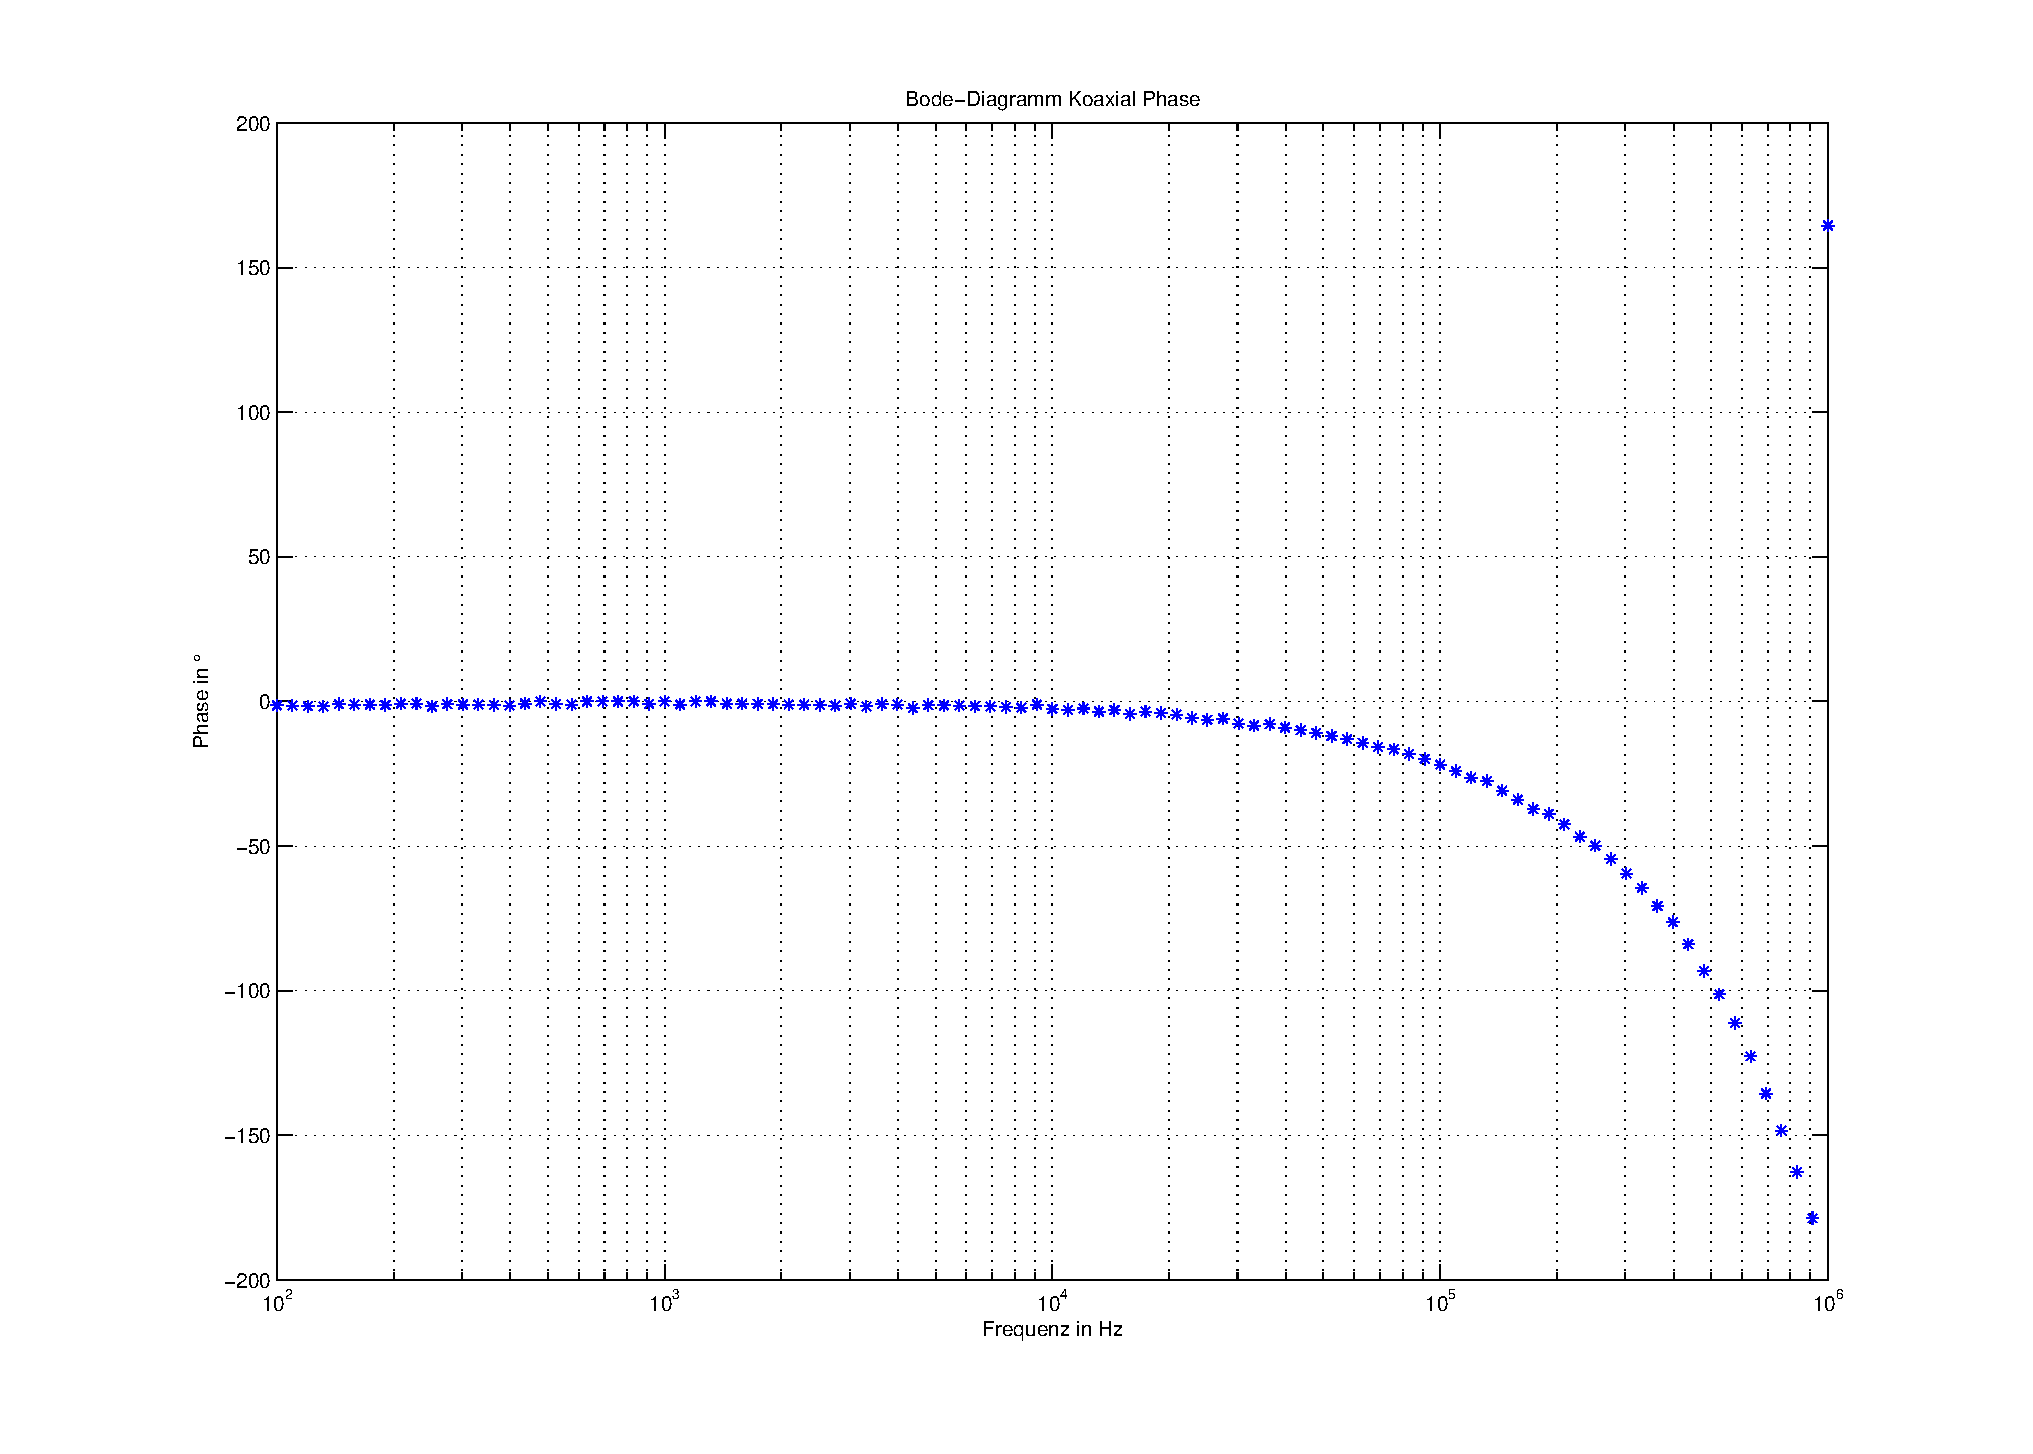
\includegraphics[scale=0.6]{./img/5d_bode_phase.eps}
    \end{center}
    \end{figure}
\end{frame}
\begin{frame}
    \frametitle{Aufgabe 5}
    \framesubtitle{Dämpfung}
    \begin{itemize}
        \item Kabel wirkt wie Tiefpassfilter
        \item Phase oszilliert stark ab $10^6 Hz$
    \end{itemize}
\end{frame}

%\chapter{Masse, Größe und Struktur der Atome} % (fold)
\label{cha:Masse,_Groesse_und_Struktur_der_Atome}
\section{Bedeutung der Atom- und Molekülphysik} % (fold)
\label{sec:Bedeutung der Atom- und Molekülphysik}
\begin{erl}{Atomphysik}
    mikroskopischer Aufbau der Materie, d.h der Struktur der Atome un ihrer
    gegenseitugen Wechselwirkung. 
\end{erl}

\begin{erl}{Ziel}
    Eigenschaften der makroskopischen Materie aus ihrem mikroskopischen Aufbau
    zu verstehen
\end{erl}

Atom- und Molekülphysik bildet die Grundlage der
\begin{itemize}
    \item Thermodynamik (für statistische Beobachtungen)
    \item Atmosphährenphysik, Meteorologie (Wetter)
    \item Festkörperphysik
    \item Astrophysik (Absorption und Emission von Strahlung)
    \item Licht-Materie Wechselwirkung
    \item Laserlicht
\end{itemize}
Atom- und Molekülphysik bildet darüber hinaus die Grundlage der Chemie und
zunehmend der Biologie und Medizin:
\begin{itemize}
    \item Einordnung der Atome im Periodensystem
    \item Molkeülbildung, -bingungen, -struktur
    \item chemische Reaktionen (Dynamit)
    \item biologische Prozesse (Photosynthese, Energieproduktion in Zellen,
    Ionentransport durch Zellmembran, Nervenleitung)
\end{itemize}
$\rar$ Molekularbiologie + Molekularmedizin

Atomphysik spielt eine wichtige Rolle in der modernen Technik
\begin{itemize}
    \item Entwicklung des Lasers (Messtechnik, Nachrichtentechnik,
    Produktionstechnik Medizin)
    \item Messtechnik (Oszillograph, Spektrographen, Tomographen)
    \item Halbleitertechnik (integrierte Schaltung)
    \item Medizintechnik (Spurenelemente ???)
    \item Umwelttechnik
    \item Energietechnik (Solarzelle, alternative Antriebstechniekn wie z.B
    Brennstoffzelle)
\end{itemize}
\begin{erl}{Atomphysik}
Ausganspunkt für die Entweicklung der Quantemechanik und damit für unseres
heutiges physikalisches Weltbild (probabilistische Beschreibung der Physik,
Heisenbergsche Unschärferelation, Welle-Teilchen-Dualismus, nicht-lokal
verschränkte Zustände)
\end{erl}
% section Wiederholung klassische Mechanik (end)

\section{Die Hohlraumstrahlung} % (fold)
\label{sec:Die_Hohlraumstrahlung}
\subsection{Herleitung der Strahlungsleistung eines schwarzen Körpers durch
Planck} % (fold)
\label{sub:Herleitung_der_Strahlungsleistung_eines_schwarzen_Körpers_durch_Plan}
Heiße Körper senden aufgrund ihrer Temperatur elektromagnetische Strahlung aus.
Die Gesetze für die spektrale Intensitätsverteilung der Wärmestrahlung erhält
man aus der Analyse eines "schwarzen Strahlers", d.h. eines schwarzen Körpers,
dessen Absorptionsvermögen $A=1$ ist. Dieser wird annährend durch einen
Hohlraum mit absorbierenden Wänden realisiert, der eine kleine Öffnung hat:
Strahlung, die durch die Öffnung eintritt, wird i.d.R vollständig absorbiert,
bevor sie wieder austreten kann ($A\simeq1$).
Wenn man die Wände des Hohlraums auf eine Temperatur $T$ heizt, wirkt die
Öffnung als Strahlungsquelle. Im thermischen Gleichgewicht ist die aus dem
Raumwinkel $d\Omega$ im Frequenzintervall $d\nu$ von der Öffnung absorbierte
Strahlungsleistung gleich der nach $d\Omega$ innerhalb $d\nu$ von der Öffnung
emittierten Strahlungsleistung:
\begin{equation*}
    \frac{d W_A}{d t}= A_{\nu} S_{\nu} d\Omega d\nu 
    =
    E_{\nu} d\Omega d\nu = \frac{d W_e}{d t}
\end{equation*}
mit $S_{\nu} = S_{\nu} \lk \nu \Omega \rk = c \cd \mu_{\nu} \lk \nu \Omega \rk $
der spektralen Strahlungsdichte des Hohlraums. Mit $A_{\nu} =1 $ folgt $E_{\nu}
= S_{\nu}$. D.h. durch Messung der aus dem Licht austretenden Strahlungsleistung
$E_{\nu}$ lässt sich die Energiedichte $\mu_{\nu} = \frac{S_{\mu}}{c}$ im
Inneren des schwarzen Körpers bestimmen. 

In einem Hohlraum können dauerhaft nur Wellen oszillieren, bei denen ein
Vielfaches der halben Wellenlange gleich der Länge des Hohlraums ist
(Eigenmoden/Eigenschwingungen):
\begin{equation*}
    n_i =  \frac{\lambda}{L_i} \qquad (i = x,y,z)
\end{equation*}
bzw.
\begin{equation*}
    k_i = \frac{2\pi}{\lambda}=n_i \frac{\pi}{L}
\end{equation*}
\begin{beis}
    $n_x = 4$    
    %BILD
\end{beis}
Wie viele solcher Eigenmoden können in einem kubischen Resonator mit
Kantenlängen $L=L_x=L_y=L_y$ existierien? Im $\vec{k}$-Raum enstrpechen die erlaubten
Eigenmoden diskreten Punkten, die ein Gitter mit Gitterkonstanten
$\frac{\pi}{L}$ (im positiven Oktanden) bestehen. Pro Einheitsvolumen im
$\vec{k}$-Raum
befinden sich $\lk \frac{\pi}{L}\rk^{-3}$ erlaubter $k$-Werte, in einer Kugel
mit Radius $k_6$ also
\begin{equation*}
    \frac{1}{8}\frac{4}{3}\pi k_6^3 \lk \frac{L^3}{\pi^3} \rk 
    = \frac{1}{6}k_6^3 \frac{V}{\pi^2}
\end{equation*}
erlaubter $k$-Werte. Da jede Mode zwei unabhangige Polarisationsrichtungen hat,
befinden sich in dieser Kugel also insgesamt $2 \cd \frac{1}{6} k_6^3
\frac{V}{\pi^2}= \frac{k_6^3}{3}\frac{V}{\pi^2}$ solcher Moden. die Zahl der
moden pro Volumeneinheit $k<k_6$ ist also
\begin{equation*}
    n= \frac{N}{V}= \frac{k_6^3}{3\pi^2}=\frac{8\pi\nu^3}{3c^3}
\end{equation*}
d.h. im Frequenzintervall $d\nu$ befinden sich folgende Anzahl von Moden:
    \begin{equation*}
    \boxed{
        n_{\nu} d\nu 
        =
        \frac{d n}{d \nu} d\nu = \frac{8 \pi \nu^2}{c^3} d\nu
        }
    \end{equation*}
Die spektrale Enegiedichte $\mu_{\nu}$ ergibt sich daraus zu:
\begin{equation*}
    \mu_{\nu} d \nu = n_{\nu} \bar{W_{\nu}(T)} d\nu
\end{equation*}
%ORDENTLICHE BARS
mit $\bar{W_{\nu}(T)}$ der von der Temperatur abhängigen mittleren Energie pro
Mode im Frequenzintervall $\left[ \nu, \nu+d\nu\right]$. Rayleigh und James
ordneten $1894$ jeder Eigenschwingung wie beim klassichen harminischen
Oszillator) die mittlere Energie $k_B T$ zu.
\begin{equation*}
\tag*{\text{(Rayleigh-Jeansches Strahlungsgesetz)}}
\boxed{
    \mu_{\nu} d\nu = \frac{8\pi\nu^2}{c^2}k_B T d\nu
    }
\end{equation*}
Aus dem Loch des Hohlraums würde also die Strahlungsleistung:
\begin{equation*}
    S_{\nu} d\nu d\Omega 
    =
    c \mu_{\nu} d\nu \frac{d\Omega}{4\pi}
    =
    c \frac{1}{4\pi} \frac{8\pi\nu^3}{c^3}k_B T d\nu d\Omega
\end{equation*}
also
\begin{equation*}
    \boxed{
    S_{\nu} d\nu d\Omega 
    =
    \frac{2\nu^2}{c^2} k_B T d\nu d\Omega
    }
\end{equation*}
emittiert werden. Für niederige Frequenzen ergibt sich gute Übereinstimmung mi
den experimentellen Ergebnissen, für hohe Frequenzen treten große Diskrepanzen
auf, für $v\rar \infty$ divergiert $S_{\nu}$ sogar (Ultraviolett-Katastrophe).

Max Planck ($1858$-$1947$) lößte dieses Problem indem er $1900$ annahm, dass
jede Eigenmode Energie nicht in beliebig kleinen Beträgen besitzt, sondern nur
in diskreten Werten ("Energiequanten"). Diese hängen von der Grequenz der
Eigenmode ab und sind immer ganzzahlige Vielfache von $h \cd \nu$, dem
kleinstmöglichen Energiequant (=Photon). Die Energie einer eigenschwingung mit
$n$ Photonen der Frequenz $\nu$ ist demnach:
\begin{equation*}
    \tag*{(Planck'sches Wirkungsquantum)}
    \boxed{
    E_n = n \cd h \nu
    }
    \quad
    \text{mit}
    \quad
    \boxed{
        h=6.625 \cd 10^{-34} Js
    }
\end{equation*}
Im thermischen Gleichgewicht ist die Wahrschenilichkeit $P(E)$, dass eine
Eigenmode die Energie $E_n$ besitzt, durch den Boltzmanfaktor
$e^{-\frac{E_n}{k_B T}}$ gegeben, die normierte Wahrscheinlichkeit also durch
\begin{equation*}
    P(E_n)
    =
    \frac{e^{-\frac{n h \nu}{k_B T}}}{\sum_{n=0}^{\infty}e^{-\frac{n h \nu}{k_B T}}}
\end{equation*}
(mit $\sum p(E_n) =1$)
Die mittlere Energie pro Eigenmode ergibt sich damit zu
\begin{equation*}
    \bar{E}_n
    =
    \sum_{n=0}^{\infty} E_n p(E_n)
    =
    \frac{\sum n k \nu e^{-\frac{nh\nu}{k_B Ta}}}{\sum e^{-\frac{nh\nu}{k_B Ta}}}
\end{equation*}
\begin{equation*}
    E_n = \frac{1}{e^{-\frac{nh\nu}{k_B Ta}}-1}
\end{equation*}
\begin{erl}{Beweis}
(mit $\beta = \frac{1}{k_B T}$)
\begin{enumerate}
    \item 
    \begin{equation*}
        \sum_{n=0}^\infty e^{-n h \nu \beta}
        =
        \frac{1}{1- e^{-h\nu\beta}}\qquad \text{(mit $\sum_{n=0}^N x^n =
        \frac{1-x^{N+1}}{1-x}$)}
    \end{equation*}
    \item
    \begin{align*}
        \sum_0^{\infty} n h \nu e^{-n h \nu \beta}
        &=
        - \frac{\p}{\p \beta} \lk \sum_{n=0}^{\infty} e^{-n h \nu \beta} \rk
        \\
        &=
        - \frac{\p}{\p \beta} \lk \frac{1}{1-e^{-h \nu \beta}} \rk \\
        &=
        \frac{h \mu e^{-h \nu \beta}}{\lk 1 - e^{-h \nu \beta} \rk^2}
    \end{align*}
\end{enumerate}
also
\begin{equation*}
    \bar{E}_n = \frac{(2)}{(1)}= \frac{h\nu}{e^{\frac{h \nu}{k_B T}} -1}
\end{equation*}
\end{erl}
Daraus folgt die spektrale Energiedichte dr Hohlraumstrahlung:
\begin{equation*}
    \tag*{\text{(Plansch'sches Strahlungsgesetz)}}
    \boxed{ 
    \mu_{\nu} (\nu) d\nu =
    \frac{8 \pi \nu^2}{c^3} \frac{h \nu}{e^{\frac{h \nu}{k_B T}}-1} d\nu
    }
\end{equation*}
\begin{bem}
    \item
    Für $h \nu \ll k_B T$ kann man den Nenner entwickeln zu 
    \begin{gather*}
       e^{\frac{h\nu}{k_B T}} \simeq 1 + \frac{k\nu}{k_B T} + \ddots \\
       e^{\frac{h\nu}{k_B T}} -1 \simeq \frac{k\nu}{k_B T} 
    \end{gather*}
    also
    \begin{equation*}
       \mu_{\nu} (\nu) = \frac{8\pi \nu^2}{c^3}k_B T \rightarrow \text{RJ!}
    \end{equation*} 
    d.h das R.J Gesetz entpuppt sich als Grenzfall des plank'schen
    Strahlungsgesetzes für kleine $\nu$.
    \item
    das beste, je gemessene Spektrum eines schwarzen Strahlers ist die von
    Reuzies und Wilson $1965$ enddeckte und $1995$ vom Satelliten Cobe
    gemessene "kosmische Hintergrundstrahlung", d.h das "Nachglühen" der vor
    ca. $13.7 Mrd$ Jahren in einem sog. "Big Bang" erfolgte Entstehung des
    Universums.
    \item
    mit $\nu = \frac{c}{\lambda}$ und $d\nu = - \frac{\nu^2}{c}d\lambda$ kann
    man das plank'sche Strahlungsgesetz auch schreiben
    \begin{equation*}
        \boxed{
            u_{\lambda} d\lambda
            =
            \frac{8\pi h c}{\lambda^5} \frac{d\lambda}{e^{\frac{hc}{\lambda k_B
            T}-1}}
        }
    \end{equation*}
    Das Maximum dieser Verstärkung ergibt sich zu
    \begin{equation*}
        \lambda_{max} = \frac{2.88 \cd 10^{-3}}{T} K \cd m
    \end{equation*}
    also
    \begin{equation*}
        \tag*{(Wiensches Verschiebungsgesetz)}
        \boxed{
            \lambda_{max} \cd T = \const
            }
    \end{equation*}
    \begin{quote}
        "Das Maximum der Energiedichte bez. der emittierten Strahlungsleistung
        eines schwarzen Körpers liegt bei einer Wellenlänge, deren Wert $\sim
        \frac{1}{T}$ ist."
    \end{quote}
    \item
    Die gesamte Energiedichte der Hohlraumstrahlung ist:
    \begin{equation*}
        u(T) = \int_{v=0}^{\infty} u_{\nu} (\nu,T) d\nu
        =
        \frac{8 \pi \h}{c^3} \int_0^{\infty} \frac{\nu^3}{e^{\frac{h\nu}{k_B
        T}}-1} d\nu
    \end{equation*}
    \begin{equation*}= \frac{8\pi^5 k_B}{15 k^3 c^3 }T^4 = T^4
        \rightarrw u(T) 
    \end{equation*}
\end{bem}
Die aus dem Loch des Hohlraums emittierte Strahlungsleistung ergibt sich daraus
zu:
\begin{gather*}
    S_{\nu} d\nu d\Omega = c \cd \frac{d\Omega}{4\pi} \frac{8 \pi h \nu^3}{c^3}
    \frac{d\nu}{e^{\frac{h\nu}{k_B T} -1}} \\
    \rar \boxed{
        S_{\nu} d\nu d\Omega 
        =
        \frac{2 h \nu^3}{c^2} \frac{d\nu d\Omega}{e^{\frac{h\nu}{k_B T}}-1}
        }
\end{gather*}
in sehr guter Übereinstimmung mit dem Experiment
\begin{erl}{Bemerkung}
Die gesamte Energiedichtestrahlung ist
\begin{align*}
    \mu(T)
    &=
    \int_{v=0}^{\infty} \mu_{\nu} (v,T) d\nu
    =
    \frac{8 \pi h}{c^3} \int \frac{\nu^3}{e^{\frac{h \nu}{k_B T}}-1} d\nu \\
    &=
    \frac{8\pi^5 k_B^4}{15 h^3 c^3}\cdot T^4 = a \cd T^4  
\end{align*}
Die von dem Oberflächenelement in $d\Omega$ emittierte Strahlung ist also
\begin{equation*}
    S(T) = c \cd a \cd T^4 \frac{d\Omega}{4\pi} \cos \vartheta
\end{equation*}
d.h die Strahlungsleistung pro Flachenelement in dem gesamten Hohlraum ist
\begin{equation*}
   I = \int S(T) d\Omega = \sigma \cd T^4 \qquad \text{ mit $\sigma = \frac{2\pi^5
   k_B^4}{15c^2 h^3} = 5.67 \cd 10^{-8} \frac{1}{K^4}\frac{W}{m^2}$}
\end{equation*}
\end{erl}
% subsection Herleitung der Strahlungsleistung eines schwarzen Körpers durch Plan (end)
\subsection{Herleitung der Planckschen Strahlungsformel nach Einstein} % (fold)
\label{sub:Herleitung_der_Planckschen_Strahlungsformel_nach_Einstein}
Max Planck ordnete $1900$ den Schwingungen des elektromagnetischen Feldes
diskrete Energiewerte zu. dies war ein mathematsiches Konstrukt, mit dem er die
ERgebnisse quantitativ verfizieren konnte. Einstein ging darüber hinaus und
ordneete den Energiequanten eine reelle Existenz zu, als sog. Photonen.

Er postulierte damit, dass Licht uaus Teilchen besteht ($\rightarrow$
Photoeffekt), d.h dass jede Welle der Frequenz $\nu$ eine anzahl von Photonen
der Eneregie $h \nu$ und den Impuls
\begin{equation*}
    \vec{p} = \hb \vec{k} = \frac{h}{2\pi} \vec{k}
\end{equation*}
besitzt. $1917$ leitete er das Planckesche Strahlungsgesetz aus der Annahme
her, dass sich Licht eines schwarzen Körpers im thermischen Gleichgewicht mit
den Wanden des schwarzen Körpers befindet, in dem die Atome Photonen
absorbieren und emittieren ($\rar$ erste quantale Beschreibung der
Licht-Materie-Wechselwirkung). Die Atome besitzen hierbei diskrete
Energieniveaus $E_1$ und $E_2$ mit $E_2 - E_1 = \Delta E = h\nu$.
\\
Drei Prozesse beschreiben die Wechselwirkung der Materie mit der
elektromagnetischen Strahlung
\begin{itemize}
    \item Absorption eines Photons
    \item spontante Emission (nach natürlicher Lebensdauer in $E_2$ 
    \item induzierte/stimulierte Emission (von Einstein einfgeführt)
\end{itemize}
Gegeben sei für ein System von $N_1$ Atomen in $E_1$ und $N_2$ Atomen in $E_2$
(mit $N_1 + N_2 = N$) im thermischen Gleichgewicht mit der Strahlung:
\\
Anzahl der Übergänge von $1 \rar 2$:
\begin{equation*}
     \dot{N}_{12} = B_{12} \cd u(\nu) \cd N_1
\end{equation*}
Anzahl der Übergänge von $2 \rar 1$:
\begin{equation*}
    \dot{N}_{21} = B_{21} u(\nu) \cd N_2 + A_{21} \cd N_2
\end{equation*}
mit $B_{12}$,$B_{21}$ und $A_{21}$ den entsprechenden Übergangsraten der
oben genannten Prozesse (=Einstein-Koeffizienten). Im thermischen Gleichgewicht
ist $\dot{N}_{12} = \dot{N}_{21}$ und
\begin{equation*}
    \frac{N_2}{N_1} = e^{-\frac{E_2 - E_1}{k_B T} = e^{-\frac{h\nu}{k_B T}}
\end{equation*}
\begin{equation*}
    u{\nu}
    =
     \frac{A_{21}}{B_{12} e^{\frac{h\nu}{k_B T}} - B_{21}}
    =
    \ddots
    =
    \frac{8 \pi h \nu^3}{c^3} \frac{1}{e^{\frac{h\nu}{k_B T}}}
\end{equation*}
% subsection Herleitung der Planckschen Strahlungsformel nach Einstein (end)
% section Die Hohlraumstrahlung (end)

% chapter Masse, Größe und Struktur der Atome (end)

    
\end{document}

%\begin{figure}[H]
%\begin{center}
%    \fbox{
%        \includegraphics{}
%    }
%\end{center}
%\end{figure}
